\section{The MCG and FPG}
    \label{s:building graphs}
We now discuss how the graph-based syntax defined in Sec.~\ref{s:syntax definition} is used to represent an MDAO problem in its entirety. This discussion is based on the MCG and the FPG.

\subsection{Maximal Connectivity Graph}
    \label{ss:MCG}
For a specified MDAO problem, the maximal connectivity graph represents every analysis tool, objective, constraint, and global input being considered, as well as every possible interconnection among them.
The definition of the MCG is given via construction.
    To construct the maximal connectivity graph, we presume that a set of analysis tools, global inputs, objectives, and constraints are provided. 
    Each of the $m$ analysis codes correspond to an index $i\in I_A$, $I_A=\{1,2,\ldots,m\}$, and are represented by an analysis block graph $G_{A_i}=(V_{A_i},E_{A_i})$.
    Each of the $n$ expression blocks correspond to an index $i\in I_E$, $I_E=\{1,2,\ldots,n\}$, and are represented by an expression block graph $G_{E_i}=(V_{E_i},E_{E_i})$.
    Finally, the global inputs are represented as a set of variable nodes $V_\txt{in}$.
    We presume that $V_\txt{in}$, each $G_{A,i}$, and each $G_{E,i}$ are given, and that any potential connection between variables is specified in the form of connection edges in the set $E_{M,\txt{con}}$. One method for defining these connections is to use a consistant variable naming convention.
    We may then construct the maximal connectivity graph $M=(V_M,E_M)$ as
    \begin{IEEEeqnarray*}{rCl}
    V_M & = & V_\txt{in} \cup \left( \bigcup_{i \in I_A} V_{A_i} \right) \cup \left( \bigcup_{i \in I_E} V_{E_i} \right), \\
    E_M & = & E_{M,\txt{con}} \cup \left( \bigcup_{i \in I_A} E_{A_i} \right)  \cup \left( \bigcup_{i \in I_E} E_{E_i} \right).
    \end{IEEEeqnarray*}
    The MCG $M$ is uniquely determined by the given set of analysis blocks, global inputs, and expression blocks. 
    In the cases where the set of global inputs is not known a priori, the process of obtaining the FPG will reveal the required inputs, as discussed subsequently.

The nodes and edges in $M$ can be partioned in sets according to their type:
\begin{equation}
V_M = V_{M,\txt{var}} \cup V_{M,\txt{mod}}, \ V_{M,\txt{var}} \cap V_{M,\txt{mod}} = \emptyset,
\end{equation}
where $V_{M,\txt{var}}$ and $V_{M,\txt{mod}}$ are the sets of variable nodes and model nodes, respecively;
\begin{equation}
E_M = E_{M,\txt{con}} \cup E_{M,\txt{mod}}, \ E_{M,\txt{con}} \cap E_{M,\txt{mod}} = \emptyset,
\end{equation}
where $ E_{M,\txt{con}}$ and $E_{M,\txt{mod}}$ are the sets of connection edges and model edges, respectively. These sets will be referenced in the process for obtaining an FPG.

\subsection{Fundamental Problem Graph}
    \label{ss:FPG}
    We now define the fundamental problem graph $F=(V_F,E_F)$ as a directed graph meeting the following conditions:
    \begin{enumerate}
    \item[(1)] $F \subset M$ and $G_{E_i} \subset F  \ \forall i \in I_E$
%    \item[(1)] $F \subset M$ and $V_\txt{out} \subset V_F$
    \item[(2)] $\displaystyle{\forall i \in I_A, \txt{ if } F \cap G_{A_i} \neq \emptyset \txt{ then } G_{A_i} \subset F}$
%    \item[(2)] $\displaystyle{\forall i \in I, \txt{ if } F \cap A_i \neq \emptyset \txt{ then } A_i \subset F}$
    \item[(3)] $\displaystyle{\forall v \in V_F \txt{ with }v \in V_{M,\txt{var}} \txt{ and }  \txt{deg}_l^-(v) \leq \txt{deg}^-(v) \leq \txt{deg}_u^-(v)}$
    \item[(4)] $\displaystyle{\forall v \in V_F \txt{ there exists a reverse path } P \subset R_F \txt{ from } x \txt{ to } v \txt{ with } x\in V_{E_i}}$
%    \item[(4)] $\displaystyle{\forall v \in V_F \txt{ there exists a reverse path } P \subset R_F \txt{ from } x \txt{ to } v \txt{ with } x\in V_\txt{out}}$
    \end{enumerate}
    %The set $I_F$ is an index set containing the indices of the analysis blocks in $F$ and it may only include the analysis blocks $A_i$ that meet requirements (2) and (6). 
    %Requirement (2) stipulates that each analysis blocks in $F$ must have at least one local output that is being used. 
    %Requirement (3) stipulates that only the global inputs that are being used should be included. 
    %Requirements (4) and (5) provide the construction of the sets of nodes and edges, respectively. 
    Condition (1) asserts that only the nodes and edges provided by the maximal connectivity graph can be used in the fundamental problem graph and that every expression block must be included. 
    Condition (2) requires that analysis blocks must be included or excluded in their entirety. 
    Condition (3) stipulates that the number of edges directed into each variable node must be within the lower and upper in-degree limits; 
    if $\txt{deg}^-(v) < \txt{deg}_l^-(v)$ the node is the location of a \emph{hole}, and if $\txt{deg}^-(v) > \txt{deg}_u^-(v)$ the node is the location of a \emph{collision}.
    Lastly, condition (4) ensures that only the nodes that are being used are included in the FPG by requiring that for every node a reverse path exists from at least one expression block to that node. 
    The reverse graph $R_F$ is obtained from $F$ by simply switching the orientation of every edge in $E_F$.

    %The set $C_F$ is a set containing connection edges representing connections. Since $C_M$ is the set of all potential connections, we must have $C_F \subset C_M$. 
    %While no other conditions are explicitly stated for $C_F$, requirement (6) is actually a requirement on both $I_F$ and $C_F$.

\subsection{Algorithm for obtaining the Fundamental Problem Graph from the MCG}
    \label{ss:obtaining FPG}
    In general, there may be zero, one, or many graphs that satisfy the FPG conditions in Sec.~\ref{ss:FPG}.
    Here, we describe an algorithm for obtaining an FPG by starting with the MCG and disconnecting connection edges until the FPG conditions are met. 
    With this approach, the problem is reduced to deciding which connection edges to remove. First, we describe a pruning subroutine used within the algorithm, and next we describe the algorithm itself.

    \begin{description}
    \item[\bf{Subroutine: Pruning}] 
        Given a digraph $G_1 = (V_1,E_1)$, let the subroutine denoted as $P_\txt{prune}$ operate on $G_1$ to produce a new digraph $G_2$ as
	\begin{equation}
	G_2 = P_\txt{prune}(G_1) = (V_2,E_2),
	\end{equation} 
	where $G_2$ now satisfies requirements (2) and (4) in Sec.~\ref{ss:FPG}.
        Pruning is accomplished by first creating the reverse graph of $G_1$, $R = (V_1,E_R)$, where
	\begin{equation}
	E_R = \{ (x,y) \st (y,x) \in E_1\}.
	\end{equation}
	Next, a new node $b$ is added to $V_1$ and edges directed from this node to each of the expression blocks are added:
    \begin{equation}
        \forall i \in I_E,\forall v \in V_{E_i}, \txt{ if } \txt{deg}^+(v)=0 \txt{ then } (b,v) \in E_R
    \end{equation}
        The set of nodes that may be reached from $b$ is constructed as
    \begin{equation}
        U = \{ v \in V_1 \st \exists P \txt{ a path from $b$ to $v$}, \ P \subset R \}.
        \end{equation}
	Because $b$ is directed into only the expression blocks, any path from $b$ necessarily provides a path from at least one expression block, which means the node is being used in the problem formulation.

        The list of analysis blocks with at least one node in $U$ is constructed as
        \begin{equation}
        I_2 = \{ i \in I_A \st V_{A_i} \cap U \neq \emptyset \}
        \end{equation}
        Any analysis block not in $I_2$ should be removed from the graph because none of its outputs contribute to the problem. Global inputs that are not being used are also removed. The set of nodes to remove is then
        \begin{equation}
        N = (V_\txt{in}\setminus U )  \cup \left( \bigcup_{i \notin I_2} V_{A_i} \right),
        \end{equation}
and the new set of nodes is created as
        \begin{equation}
        V_2 = V_1 \setminus N.
        \end{equation}
        Edges involving the removed nodes are also deleted as
        \begin{equation}
        E_2 = E_1 \setminus \{ (x,y) \st x \in N \txt{ or } y \in N  \}.
        \end{equation}
        The set of connection edges can be extracted by considering only edges whos endpoints are not in the same analysis block:
        \begin{equation}
        E_{2,\txt{con}} = \{(x,y) \in V_{2} \st \sim(x \in V_{A_i} \txt{ and } y \in V_{A_i} \txt{ for some } i \in I_2)\}.
        \end{equation}
        %which means $C_2 \cap V_{A_i} = \emptyset  \ \forall i \in I_1$, and $E_2 = C_2 \cup \left( \bigcup_{i \in I_1} E_{A_i} \right)$. 
\end{description}

\noindent The algorithm for obtaining an FPG can now be described as follows:
\begin{description}
    \item[\bf{Step 1: Holes}] 
        The first step is to detect holes and disconnect the first set of connection edges downstream of them, as indicated in Fig.~\ref{f:hole}. 
        These connection edges are removed because they represent output variables which cannot be determined because the analysis function does not have adequate inputs. 

        To begin the process, an initial graph is created as a pruned copy of the MCG
        \begin{equation}
        F_0 = P_\txt{prune}(M),
        \end{equation}
        where $F_0 = (V_{F_0},E_{F_0})$, and $C_{F_0,\txt{con}}$ is also obtained as described. 
        The set of variable nodes which are holes is identified as
        \begin{equation}
        H = \{v \in V_{F_0} \st v \in V_{M,\txt{var}} \txt{ and } \txt{deg}^-(v) < \txt{deg}_l^-(v) \},
        \end{equation}
        which is the set of variable nodes with fewer incoming edges than are allowed by the lower indegree limit.
        The updated set of connection edges is then created by removing the edges preceding or succeeding the analysis block:
        \begin{equation}
        E_{F_1,\txt{con}} = E_{F_0,\txt{con}} \setminus \{(x,y) \in E_{F_0,\txt{con}} \st x \in V_{A_i} \txt{ or } y \in V_{A_i}, \txt{ and } H\cap V_{A_i} \neq \emptyset \}.
    \end{equation}
Because removing these edges can create new holes, this step must be repeated until no additional holes are found.
        If the hole identification step identifies a variable node in an expression block as hole, meaning $V_{E_i} \cap H \neq \emptyset$ for some $i \in I_E$, then the algorithm terminates because an FPG cannot be obtained. 

If this step finishes without finding a hole in an expression block, it is guaranteed that an FPG can be obtained because $F_1$ now satisfies all four conditions from Sec.~\ref{ss:FPG} expect for (3), which requires there to be no holes or collisions in the graph. Since no more holes remain, and collisions can always be resolved without producing a hole, (see Table \ref{t:variable node classification}), then it is guaranteed than an FPG can be obtained.

    \begin{figure}[htb!]
        \begin{center}
        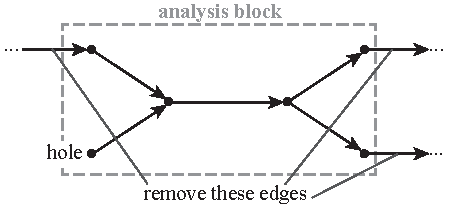
\includegraphics[width=3in]{images/analysis_block_hole}
        \end{center}
        \vspace{-20pt}
    \caption{Example variable node indicating a hole.}
    \label{f:hole}
    \end{figure}

    \item[\bf{Step 2: Collisions}] 
        The second step is to detect collisions and to disconnect precisely the number of connection edges required such that all collisions are resolved without introducting holes. 
        The set of variable nodes at which collisions occur is 
    \begin{equation}
    S_\txt{nodes} = \{v \in V_{M,\txt{var}} \st \txt{deg}^-(v) > \txt{deg}_u^-(v) \}.
    \end{equation}
    For each collision node we can construct a set containing the edges directed into the node. The set containing all of these sets is constructed as
    \begin{equation}
        S_\txt{edges} = \big \{ \{(x,y) \in E_M\} \ \big| \ y \in S_\txt{nodes} \big \}
    \end{equation}
    Let $J=\{1,2,\ldots,|S_\txt{edges}|\}$ be an indexing set for $S_\txt{edges}$ such that each $S_{\txt{edges},j}$ corresponds to a set in $S_\txt{edges}$ for $j \in J$. 
    An example collision is shown in Fig.~\ref{f:collision} to exemplify the definition of $S_{\txt{edges},j}$. 
    We can assume that $J$ also indexes $S_\txt{nodes}$ because there is a one--to--one correspondence between the elements in $S_\txt{nodes}$ and the elements in $S_\txt{edges}$ (which are sets). 
    We may then construct sets of edges as
    \begin{equation}
    B_j = \big \{e_k \in S_{\txt{edges},j} \st k \in \{1,2,\ldots,K\} \txt{ with } \txt{deg}_u^-(v_j) \leq K \leq \txt{deg}_u^-(v_j) \big \}, \ j \in J,
    \end{equation}
        which means that each set $B_j$ is constructed from the set $S_{\txt{edges},j}$ by taking only as many edges as are allowed by the upper and lower indegree limits of $v_j$.  
The construction of each $B_j$ corresponds to making a decision about which edges to include and which edges not to include. 
%An upper bound on the number of such decisions that need to be made is 
%\begin{equation}
%\prod_{j \in J} 	
%	\begin{pmatrix}
%		|S_{\txt{edges},j}| \\
%		\txt{deg}_u^-(v_j)
%	\end{pmatrix}
%\end{equation}
%where $(:)$ refers to standard $n$-choose-$k$ notation.
Let the new set of connection edges be
    \begin{equation}
    E_{F_2,\txt{con}} = \{ e \in E_{F_1,\txt{con}} \st e \in B_j \txt{ for some } j \in J\}.
    \end{equation}
The set of all edges is created by removing the connection edges not in $E_{F_2,\txt{con}}$:
    \begin{equation}
    E_{F,2} = E_{F_0} \setminus (E_{M,\txt{con}} \setminus E_{F_2,\txt{con}}),
    \end{equation}
    which gives
    \begin{equation}
    F_2 = (V_{F_0},E_{F,2}).
    \end{equation}
    \begin{figure}[htb!]
        \begin{center}
        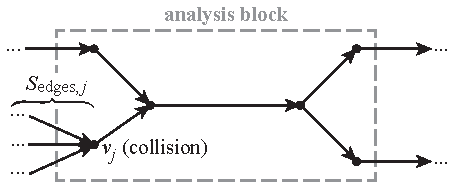
\includegraphics[width=3in]{images/analysis_block_collision}
        \end{center}
        \vspace{-20pt}
    \caption{Example variable node indicating a collision.}
    \label{f:collision}
    \end{figure}

    \item[\bf{Step 3: Finalize}] 
        The third and final step is to prune the graph a final time to exclude any analysis blocks that became unneeded after the collisions were resolved:
    \begin{equation}
        F = P_\txt{prune}(F_2),
    \end{equation}
        with $F = (V_F,E_F)$.
        The indices of the analysis blocks implemented in the FPG can then be found as
    \begin{equation}
        I_F = \{ i \in I_A \st G_{A_i} \subset F \}.
    \end{equation}
%       \begin{
%       \begin{equation}
%       I_F =  \{i \in I \ | \ \exists v \in V_{A_i} \txt{ such that }  t_\txt{node}(E_{F,2}^{-1}(v))=\txt{`model'} \txt{ and } \txt{deg}^+(v) > 0 \},
%       \end{equation}
%       where the degree is calculated with respect to $F_2$. 
%       This set excludes both the analysis blocks that were unused in the original MCG and those that became unused in step 1 or step 2.
%
%       The set of used global inputs is constructed as
%       \begin{equation}
%       V_{\txt{in},F} = \big\{v \in V_\txt{in} \ \big| \ |\{(x,y) \in E_{F,2}(v) \st y \in V_{A_i} \txt{ for } i \in I_F  \}| > 1 \big\},
%       \end{equation}
%       which requires that at least two edges directed out of the nodes in $V_{\txt{in},F}$ must be to the analysis blocks indexed by $I_F$.
%
%       Finally, the set of nodes and edges describing a fundamental problem graph is given by
%       \begin{equation}
%       V_F = V_{\txt{in},F} \cup V_\txt{out} \cup \left( \bigcup_{i \in I_F} V_{A_i} \right),
%       \end{equation}
%       \begin{equation}
%       C_{F} = \{ (x,y) \in C_{F,2} \st x,y \in V_F\},
%       \end{equation}
%       \begin{equation}
%       E_F = C_F \cup \left( \bigcup_{i \in I_F} E_{A_i} \right),
%       \end{equation}
%       \begin{equation}
%       F = (V_F,E_F).
%       \end{equation}

    \end{description}

This algorithm will always provide an FPG if one exists. If an FPG does not exist, the limiting factors preventing a valid formulation are revealed.

\subsection{Suggested Process for Using the FPG Algorithm}
\label{ss:process}
Section \ref{ss:obtaining FPG} provided an algorithm for obtaining an FPG from the given MCG. However, if an FPG cannot be obtained, this algorithm can be applied as part of a larger process in which the designer changes the problem or the supplied analyses to attempt to obtain an FPG. The following steps detail the suggested procedure for obtaining an FPG:
\begin{enumerate}
\item[\bf{(A)}] Begin with a set of global inputs, analysis codes, objectives, and constraints.
\item[\bf{(B)}] Build the MCG as described in Sec.~\ref{ss:MCG}.
\item[\bf{(C)}] Set indegree limits for variable nodes representing local inputs as described in Sec.~\ref{s:indegree-outdegree} and Table \ref{t:variable node classification}
\item[\bf{(D)}] Run the FPG algorithm described in Sec.~\ref{ss:obtaining FPG}. If a valid FPG is unattainable:
		\begin{enumerate}
\item Change the MCG by adding analysis blocks and/or global inputs, which means identifying new analyses to include in a potential MDAO workflow.
\item Change indegree limits (see Table \ref{t:variable node classification}).
\end{enumerate}
\item[\bf{(E)}] Repeat from step (A) until an FPG is obtained.
\end{enumerate}